\subsection{Probability Spaces and Event Algebra}
% Probability spaces, events, random variables, distributions, pushforward measures, independence.

Probability assigns numbers to experimental outcomes; measure theory specifies which subsets are events.

\begin{definition} \label{def:probability-space-random-variable-law}\label{def:sample-space-events-and-probability-space} \hlt{Sample Spaces, Events, and Probability Spaces}
\begin{enumerate}[label=(\roman*)]
\setlength{\itemsep}{0pt}
\item A \hlt{sample space} is a set $\Omega$ of possible outcomes.
\item An \hlt{outcome} or \hlt{realization} is a point $\omega\in\Omega$.
\item An \hlt{event} is a subset $A\subseteq\Omega$; the admissible events form a \hlt{$\sigma$-algebra} $\mathcal{F}\subseteq\mathcal{P}(\Omega)$.
\item A \hlt{probability measure} on $(\Omega,\mathcal{F})$ is a measure $\mathbb{P}:\mathcal{F}\to[0,1]$ with $\mathbb{P}(\Omega)=1$.
\item The triple $(\Omega,\mathcal{F},\mathbb{P})$ is a \hlt{probability space}.
\end{enumerate}
\hlt{Key Insight}: Probability is countably additive size normalized so that the whole sample space has mass $1$.
\end{definition}

\begin{method} \label{meth:first-sample-spaces} \hlt{Sample Space Construction Method}\\
Choose $\Omega$ as the set of complete outcomes and encode the target condition as an event $A\subseteq\Omega$:
\begin{enumerate}[label=(\roman*)]
\setlength{\itemsep}{0pt}
\item \hlt{Finite product method}: for $m$ discrete trials with state set $S$, use $\Omega=S^m$ and coordinate constraints.\\
For two coin tosses, $S=\{H,T\}$, $\Omega=S^2$, and first toss heads gives $A=\{\omega\in\Omega:\omega_1=H\}=\{HH,HT\}$.
\item \hlt{Interval method}: for real-valued measurements, use $\Omega=\R$ and translate inequalities into intervals.\\
$10<\omega\leq23$ gives $A=(10,23]$.
\item \hlt{Cylinder method}: for infinite sequences with state set $S$, use $\Omega=S^{\N}$ and constrain finitely many coordinates; for coin tosses, $S=\{H,T\}$ and first head on toss $3$ gives $A=\{\omega\in\Omega:\omega_1=T,\omega_2=T,\omega_3=H\}$.
\end{enumerate}
\end{method}

\begin{example} \label{ex:introductory-sample-spaces-and-events} \hlt{Introductory Sample Spaces and Events}
\begin{enumerate}[label=(\roman*)]
\setlength{\itemsep}{0pt}
\item If a commute passes three traffic lights, each with outcome stop $s$ or continue $c$, then $\Omega=\{c,s\}^3$. The event that the first light is a stop is $\{sss,ssc,scc,scs\}$.
\item If a print queue length is modeled as random, one possible sample space is $\Omega=\{0,1,2,\ldots\}$; with a known capacity $N$, one may instead use $\Omega=\{0,1,\ldots,N\}$.
\item If the measured waiting time between events is nonnegative, a natural sample space is $\Omega=[0,\infty)$.
\end{enumerate}
\hlt{Key Insight}: Choose $\Omega$ at the event resolution needed.
\end{example}

\begin{definition} \label{def:event-algebra-indicators-and-monotone-events} \hlt{Event Algebra, Indicators, and Monotone Events}
\begin{enumerate}[label=(\roman*)]
\setlength{\itemsep}{0pt}
\item For $A\in\mathcal{F}$, the \hlt{complement} is $A^c\defeq\Omega\setminus A$.
\item For $A,B\in\mathcal{F}$, the \hlt{union} and \hlt{intersection} are $A\cup B$ and $A\cap B$.
\item For $A,B\in\mathcal{F}$, the \hlt{difference} is $A\setminus B\defeq A\cap B^c$.
\item \hlt{Commutativity}: $A\cup B=B\cup A$ and $A\cap B=B\cap A$.
\item \hlt{Associativity}: $(A\cup B)\cup C=A\cup(B\cup C)$ and $(A\cap B)\cap C=A\cap(B\cap C)$.
\item \hlt{Distributivity}: $A\cap(B\cup C)=(A\cap B)\cup(A\cap C)$ and $A\cup(B\cap C)=(A\cup B)\cap(A\cup C)$.
\item \hlt{De Morgan laws}: $(A\cup B)^c=A^c\cap B^c$ and $(A\cap B)^c=A^c\cup B^c$.
\item Events $(A_i)_{i\in I}$ are \hlt{disjoint} or \hlt{mutually exclusive} if $A_i\cap A_j=\emptyset$ for $i\neq j$.
\item Events $(A_i)_{i\in I}$ form a \hlt{partition} of $\Omega$ if $A_i\cap A_j=\emptyset$ for $i\neq j$ and $\bigcup\limits_{i\in I}A_i=\Omega$.
\item The \hlt{indicator} of $A\in\mathcal{F}$ is $\mathbf{1}_A:\Omega\to\{0,1\}$, where $\mathbf{1}_A(\omega)=1$ for $\omega\in A$ and $\mathbf{1}_A(\omega)=0$ for $\omega\notin A$.
\item A sequence $(A_n)$ is \hlt{increasing} to $A$, written $A_n\uparrow A$, if $A_1\subseteq A_2\subseteq\cdots$ and $A=\bigcup\limits_{n\geq1}A_n$.
\item A sequence $(A_n)$ is \hlt{decreasing} to $A$, written $A_n\downarrow A$, if $A_1\supseteq A_2\supseteq\cdots$ and $A=\bigcap\limits_{n\geq1}A_n$.
\end{enumerate}
\end{definition}

\begin{proposition} \label{prop:indicator-event-algebra} \hlt{Indicator Algebra for Unions and Intersections}\\
For events $A,B\in\mathcal{F}$: $\mathbf{1}_{A\cap B}=\mathbf{1}_A\mathbf{1}_B=\min\{\mathbf{1}_A,\mathbf{1}_B\}$, and $\mathbf{1}_{A\cup B}=\max\{\mathbf{1}_A,\mathbf{1}_B\}$.
\begin{proof}
Fix $\omega\in\Omega$ and set $a\defeq\mathbf{1}_A(\omega)$, $b\defeq\mathbf{1}_B(\omega)$. Then $a,b\in\{0,1\}$, $\mathbf{1}_{A\cap B}(\omega)=ab=\min\{a,b\}$, and $\mathbf{1}_{A\cup B}(\omega)=\max\{a,b\}$. Since $\omega$ was arbitrary, the identities hold pointwise.\\
\hlt{Structural Commentary}: Boolean operations on events become arithmetic operations on $0$-$1$ variables.\\
\hlt{Key Insight}: Indicators let event algebra be manipulated inside sums and expectations.
\end{proof}
\end{proposition}

\begin{figure}[H]
  \centering
  % Source integration: simplified redraw of the Venn diagrams for union and
% intersection from the attached probability chapter screenshots.
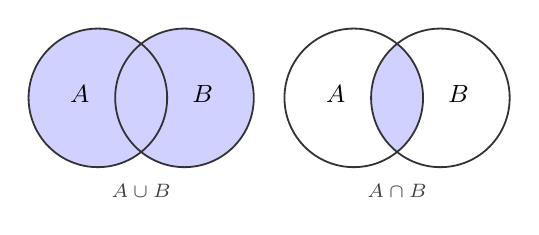
\begin{tikzpicture}[
  every node/.style={font=\small},
  set circle/.style={draw=black!80, line width=0.65pt},
  shade/.style={fill=blue!18},
  label/.style={font=\scriptsize, text=black!75}
]
  \begin{scope}
    \fill[shade] (-0.55,0) circle (0.88);
    \fill[shade] (0.55,0) circle (0.88);
    \draw[set circle] (-0.55,0) circle (0.88);
    \draw[set circle] (0.55,0) circle (0.88);
    \node at (-0.78,0.05) {$A$};
    \node at (0.78,0.05) {$B$};
    \node[label] at (0,-1.18) {$A\cup B$};
  \end{scope}

  \begin{scope}[xshift=3.25cm]
    \begin{scope}
      \clip (-0.55,0) circle (0.88);
      \fill[shade] (0.55,0) circle (0.88);
    \end{scope}
    \draw[set circle] (-0.55,0) circle (0.88);
    \draw[set circle] (0.55,0) circle (0.88);
    \node at (-0.78,0.05) {$A$};
    \node at (0.78,0.05) {$B$};
    \node[label] at (0,-1.18) {$A\cap B$};
  \end{scope}
\end{tikzpicture}

  \caption{Set operations become event operations in a probability space.}
  \label{fig:venn-union-intersection-probability}
\end{figure}

\begin{example} \label{ex:monotone-event-limits-on-real-line} \hlt{Endpoint Sensitivity in Monotone Limits}\\
Let $\Omega=\R$.
\begin{enumerate}[label=(\roman*)]
\setlength{\itemsep}{0pt}
\item If $A_i=[0,\frac{1}{i}]$, then $\bigcup\limits_{i=1}^{\infty}A_i=[0,1]$ and $\bigcap\limits_{i=1}^{\infty}A_i=\{0\}$.
\item If $A_i=(0,\frac{1}{i})$, then $\bigcup\limits_{i=1}^{\infty}A_i=(0,1)$ and $\bigcap\limits_{i=1}^{\infty}A_i=\emptyset$.
\end{enumerate}
\hlt{Key Insight}: Monotone set limits remember whether boundary points are included.
\end{example}

\begin{proposition} \label{prop:probability-axiom-consequences} \hlt{First Consequences of the Probability Axioms}\\
For events $A,B\in\mathcal{F}$:
\begin{enumerate}[label=(\roman*)]
\setlength{\itemsep}{0pt}
\item \hlt{Null event}: $\mathbb{P}(\emptyset)=0$.
\item \hlt{Monotonicity}: $A\subseteq B\Rightarrow\mathbb{P}(A)\leq\mathbb{P}(B)$.
\item \hlt{Bounds}: $0\leq\mathbb{P}(A)\leq1$.
\item \hlt{Complement}: $\mathbb{P}(A^c)=1-\mathbb{P}(A)$.
\item \hlt{Disjoint additivity}: $A\cap B=\emptyset\Rightarrow\mathbb{P}(A\cup B)=\mathbb{P}(A)+\mathbb{P}(B)$.
\item \hlt{Two-set inclusion-exclusion}: $\mathbb{P}(A\cup B)=\mathbb{P}(A)+\mathbb{P}(B)-\mathbb{P}(A\cap B)$.
\end{enumerate}
\begin{proof}
\begin{enumerate}[label=(\roman*)]
\setlength{\itemsep}{0pt}
\item Countable additivity on $\Omega=\Omega\sqcup\emptyset\sqcup\emptyset\sqcup\cdots$ gives $1=1+\sum\limits_{n\geq1}\mathbb{P}(\emptyset)$, hence $\mathbb{P}(\emptyset)=0$.
\item If $A\subseteq B$, then $B=A\sqcup(B\setminus A)$, so $\mathbb{P}(B)=\mathbb{P}(A)+\mathbb{P}(B\setminus A)\geq\mathbb{P}(A)$.
\item Since $\emptyset\subseteq A\subseteq\Omega$, (i) and (ii) give $0=\mathbb{P}(\emptyset)\leq\mathbb{P}(A)\leq\mathbb{P}(\Omega)=1$.
\item Since $\Omega=A\sqcup A^c$, $1=\mathbb{P}(\Omega)=\mathbb{P}(A)+\mathbb{P}(A^c)$, so $\mathbb{P}(A^c)=1-\mathbb{P}(A)$.
\item If $A\cap B=\emptyset$, then $A\cup B=A\sqcup B$, so $\mathbb{P}(A\cup B)=\mathbb{P}(A)+\mathbb{P}(B)$.
\item Decompose $A\cup B=(A\setminus B)\sqcup(A\cap B)\sqcup(B\setminus A)$, $A=(A\setminus B)\sqcup(A\cap B)$, and $B=(A\cap B)\sqcup(B\setminus A)$.\\
Hence $\mathbb{P}(A\cup B)=\mathbb{P}(A)+\mathbb{P}(B)-\mathbb{P}(A\cap B)$.
\end{enumerate}
\hlt{Structural Commentary}: The algebraic identities are set partitions in disguise.\\
\hlt{Key Insight}: Split overlapping sets into disjoint pieces before adding probabilities.
\end{proof}
\end{proposition}

\begin{example} \label{ex:two-coin-inclusion-exclusion} \hlt{Two Coin Tosses and Inclusion-Exclusion}\\
Let $\Omega=\{HH,HT,TH,TT\}$ with $\mathbb{P}(\{\omega\})=\frac{1}{4}$ for all $\omega\in\Omega$. Set $H_1=\{HH,HT\}$ and $H_2=\{HH,TH\}$.\\
Since $H_1\cap H_2=\{HH\}$, $\mathbb{P}(H_1\cup H_2) =\mathbb{P}(H_1)+\mathbb{P}(H_2)-\mathbb{P}(H_1\cap H_2) =\frac12+\frac12-\frac14 =\frac34$.
\end{example}

\begin{proposition} \label{prop:three-set-inclusion-exclusion-and-bonferroni} \hlt{Three-Set Inclusion-Exclusion and Bonferroni}\\
For events $A,B,C\in\mathcal{F}$:
\begin{enumerate}[label=(\roman*)]
\setlength{\itemsep}{0pt}
\item $\mathbb{P}(A\cup B\cup C)=\mathbb{P}(A)+\mathbb{P}(B)+\mathbb{P}(C)-\mathbb{P}(A\cap B)-\mathbb{P}(A\cap C)-\mathbb{P}(B\cap C)+\mathbb{P}(A\cap B\cap C)$.
\item $\mathbb{P}(A\cap B)\geq \mathbb{P}(A)+\mathbb{P}(B)-1$.
\end{enumerate}
\begin{proof}
\begin{enumerate}[label=(\roman*)]
\setlength{\itemsep}{0pt}
\item Let $U=A\cup B$. Then $A\cup B\cup C=U\cup C$ and $U\cap C=(A\cap C)\cup(B\cap C)$.\\
By two-set inclusion-exclusion, $\mathbb{P}(U\cup C)=\mathbb{P}(U)+\mathbb{P}(C)-\mathbb{P}(U\cap C)$, $\mathbb{P}(U)=\mathbb{P}(A)+\mathbb{P}(B)-\mathbb{P}(A\cap B)$,\\
and $\mathbb{P}(U\cap C)=\mathbb{P}(A\cap C)+\mathbb{P}(B\cap C)-\mathbb{P}(A\cap B\cap C)$. Substitution gives (i).
\item Since $\mathbb{P}(A\cup B)\leq1$ and $\mathbb{P}(A\cup B)=\mathbb{P}(A)+\mathbb{P}(B)-\mathbb{P}(A\cap B)$, rearrange.
\end{enumerate}
\hlt{Structural Commentary}: Inclusion-exclusion alternates between overcounting and correcting overlaps.\\
\hlt{Key Insight}: Bonferroni inequalities are one-sided forms of inclusion-exclusion.
\end{proof}
\end{proposition}

\begin{theorem} \label{thm:probability-continuity-monotone-events} \hlt{Continuity of Probabilities}
\begin{enumerate}[label=(\roman*)]
\setlength{\itemsep}{0pt}
\item \hlt{Continuity from below}: if $A_n\uparrow A$, then $\lim\limits_{n\to\infty}\mathbb{P}(A_n)=\mathbb{P}(A)$.
\item \hlt{Continuity from above}: if $A_n\downarrow A$, then $\lim\limits_{n\to\infty}\mathbb{P}(A_n)=\mathbb{P}(A)$.
\end{enumerate}
\begin{proof}
\begin{enumerate}[label=(\roman*)]
\setlength{\itemsep}{0pt}
\item Set $B_1=A_1$ and $B_n=A_n\setminus A_{n-1}$ for $n\geq2$. Then $(B_n)$ is disjoint, $A_n=\bigcup\limits_{j=1}^{n}B_j$, and $A=\bigcup\limits_{j=1}^{\infty}B_j$, so countable additivity gives $\mathbb{P}(A_n)=\sum\limits_{j=1}^{n}\mathbb{P}(B_j)\to\sum\limits_{j=1}^{\infty}\mathbb{P}(B_j)=\mathbb{P}(A)$.
\item Set $C_n=A_1\setminus A_n$. Then $C_n\uparrow A_1\setminus A$, so (i) gives $\mathbb{P}(C_n)\to\mathbb{P}(A_1\setminus A)$; since $A_1=A_n\sqcup C_n$ and $A_1=A\sqcup(A_1\setminus A)$, finite additivity gives $\mathbb{P}(A_n)=\mathbb{P}(A_1)-\mathbb{P}(C_n)\to\mathbb{P}(A_1)-\mathbb{P}(A_1\setminus A)=\mathbb{P}(A)$.
\end{enumerate}
\hlt{Structural Commentary}: Monotone limits convert countable additivity into limit rules.\\
\hlt{Key Insight}: Increasing uses increments; decreasing uses complements.
\end{proof}
\end{theorem}

\begin{definition} \label{def:limsup-liminf-events} \hlt{Events Occurring Infinitely Often and Eventually Always}\\
For events $(A_n)_{n\geq1}$:
\begin{enumerate}[label=(\roman*)]
\setlength{\itemsep}{0pt}
\item \hlt{Tail union}: $B_n\defeq\bigcup\limits_{i=n}^{\infty}A_i$.
\item \hlt{Tail intersection}: $C_n\defeq\bigcap\limits_{i=n}^{\infty}A_i$.
\item \hlt{Limsup}: $\limsup\limits_{n\to\infty}A_n\defeq\bigcap\limits_{n=1}^{\infty}B_n=\bigcap\limits_{n=1}^{\infty}\bigcup\limits_{i=n}^{\infty}A_i$.
\item \hlt{Liminf}: $\liminf\limits_{n\to\infty}A_n\defeq\bigcup\limits_{n=1}^{\infty}C_n=\bigcup\limits_{n=1}^{\infty}\bigcap\limits_{i=n}^{\infty}A_i$.
\item \hlt{Infinitely often}: $\omega\in\limsup\limits_nA_n$ iff $\omega\in A_n$ for infinitely many $n$.
\item \hlt{Eventually always}: $\omega\in\liminf\limits_nA_n$ iff $\omega\in A_n$ for all but finitely many $n$.
\end{enumerate}
\end{definition}

\begin{proposition} \label{prop:event-limsup-liminf-monotonicity} \hlt{Tail Monotonicity}\\
For events $(A_n)_{n\geq1}$ with tail union $B_n$ and tail intersection $C_n$:
\begin{enumerate}[label=(\roman*)]
\setlength{\itemsep}{0pt}
\item \hlt{Tail unions}: $B_{n+1}\subseteq B_n$ for all $n$, hence $B_n\downarrow\bigcap\limits_{n\geq1}B_n$.
\item \hlt{Tail intersections}: $C_n\subseteq C_{n+1}$ for all $n$, hence $C_n\uparrow\bigcup\limits_{n\geq1}C_n$.
\end{enumerate}
\begin{proof}
\begin{enumerate}[label=(\roman*)]
\setlength{\itemsep}{0pt}
\item Since $\{i:i\geq n+1\}\subseteq\{i:i\geq n\}$, $B_{n+1}=\bigcup\limits_{i=n+1}^{\infty}A_i\subseteq\bigcup\limits_{i=n}^{\infty}A_i=B_n$.
\item Since $\{i:i\geq n+1\}\subseteq\{i:i\geq n\}$, $C_n=\bigcap\limits_{i=n}^{\infty}A_i\subseteq\bigcap\limits_{i=n+1}^{\infty}A_i=C_{n+1}$.
\end{enumerate}
\hlt{Structural Commentary}: Tail shifts turn recurrence and permanence into monotone limits.\\
\hlt{Key Insight}: Tail unions track recurrence; tail intersections track permanence.
\end{proof}
\end{proposition}

\begin{proposition} \label{prop:union-bound-and-full-probability-intersections} \hlt{Union Bound and Countable Intersections of Almost-Sure Events}\\
For events $(A_n)_{n\geq1}$:
\begin{enumerate}[label=(\roman*)]
\setlength{\itemsep}{0pt}
\item \hlt{Union bound}: $\mathbb{P}(\bigcup\limits_{n=1}^{\infty}A_n)\leq\sum\limits_{n=1}^{\infty}\mathbb{P}(A_n)$.
\item \hlt{Countable almost-sure intersection}: if $\mathbb{P}(A_n)=1$ for all $n$, then $\mathbb{P}(\bigcap\limits_{n=1}^{\infty}A_n)=1$.
\end{enumerate}
\begin{proof}
\begin{enumerate}[label=(\roman*)]
\setlength{\itemsep}{0pt}
\item Set $B_n\defeq A_n\setminus\bigcup\limits_{j<n}A_j$. Then $(B_n)$ is disjoint, $\bigcup\limits_nB_n=\bigcup\limits_nA_n$, and $B_n\subseteq A_n$.\\
Hence $\mathbb{P}(\bigcup\limits_nA_n)=\sum\limits_n\mathbb{P}(B_n)\leq\sum\limits_n\mathbb{P}(A_n)$.
\item If $\mathbb{P}(A_n)=1$ for all $n$, then $\mathbb{P}(A_n^c)=0$ for all $n$.\\
By (i), $\mathbb{P}((\bigcap\limits_nA_n)^c)=\mathbb{P}(\bigcup\limits_nA_n^c)\leq\sum\limits_n\mathbb{P}(A_n^c)=0$, so $\mathbb{P}(\bigcap\limits_nA_n)=1$.
\end{enumerate}
\hlt{Structural Commentary}: Countable subadditivity is countable additivity after disjointization.\\
\hlt{Key Insight}: Almost sure statements survive countable intersections.
\end{proof}
\end{proposition}
